\input{../doc}
\input{../preamb}

\begin{document}
Du skal ha kompetanse om
\begin{itemize}
	\item begrepene temperatur $T$ og varme $Q$
	\item begrepet trykk $P$
	\item den ideelle gassloven
	\item termodynamikkens 1. lov $\Delta U$ $=$ $\Delta Q$ + $\Delta W$
	\item termodynamikkens 2. lov $\Delta S$ $\geq$ $0$
	\item spesifikk varmekapasitet og faseoverganger
	\item virkningsgrad $\eta$ $=$ $\frac{P_{\text{nyttbar}}}{P_{\text{tilført}}}$
\end{itemize}



\section{Temperatur og varme}
\textbf{Temperatur} ($T$) er et mål på den indre kinetiske energien i et stoff. \\ \vsk

Vi bruke Kelvin (K) istedenfor celsius ($^\text{o}$C) som temperaturskala.

\begin{figure}[H]
\centering
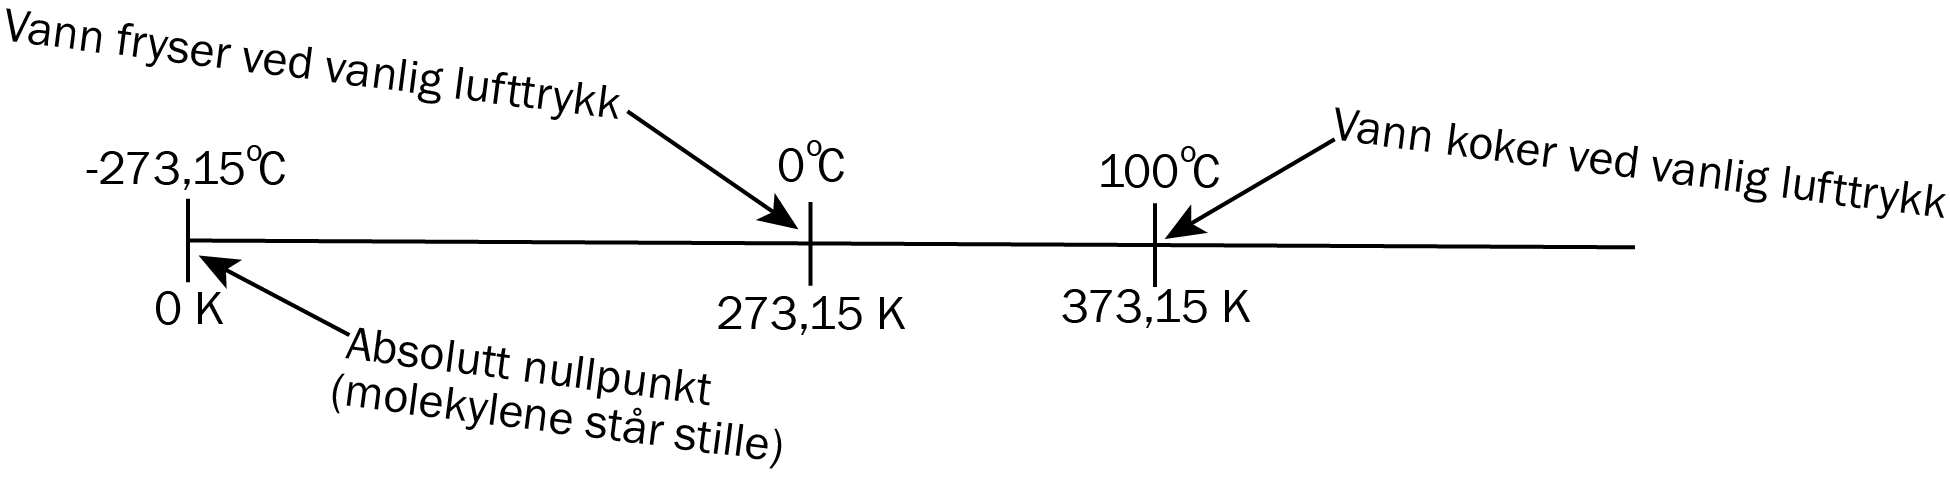
\includegraphics[width=11cm]{Skala}
\end{figure}

Sammenhengen mellom gjennomsnittlig kinetisk energi til molekylene og temperaturen er henholdsvis
\[ E_k = \frac{3}{2}kT \;\;\; \text{ og } \;\;\; E_k = \frac{5}{2} kT \]
for en én-atomig og to-atomig gass. Konstanten $k$ $=$ 1,38 $\cdot$ 10$^{-23}$ J/K er Boltzmass-konstanten. \\ \vsk

\textbf{Varme} ($Q$) er energi som går fra et sted til et annet sted på grunn av temperturforskjell mellom de to stedene. \\ \vsk

\merk[]{Bruken av begrepene "temperatur" og "varme" i hverdagsspråket og i f.eks. aviser er ofte feil!}


Eksempel på feil bruk av begrepene "temperatur" og "varme":
\begin{figure}[H]
\centering
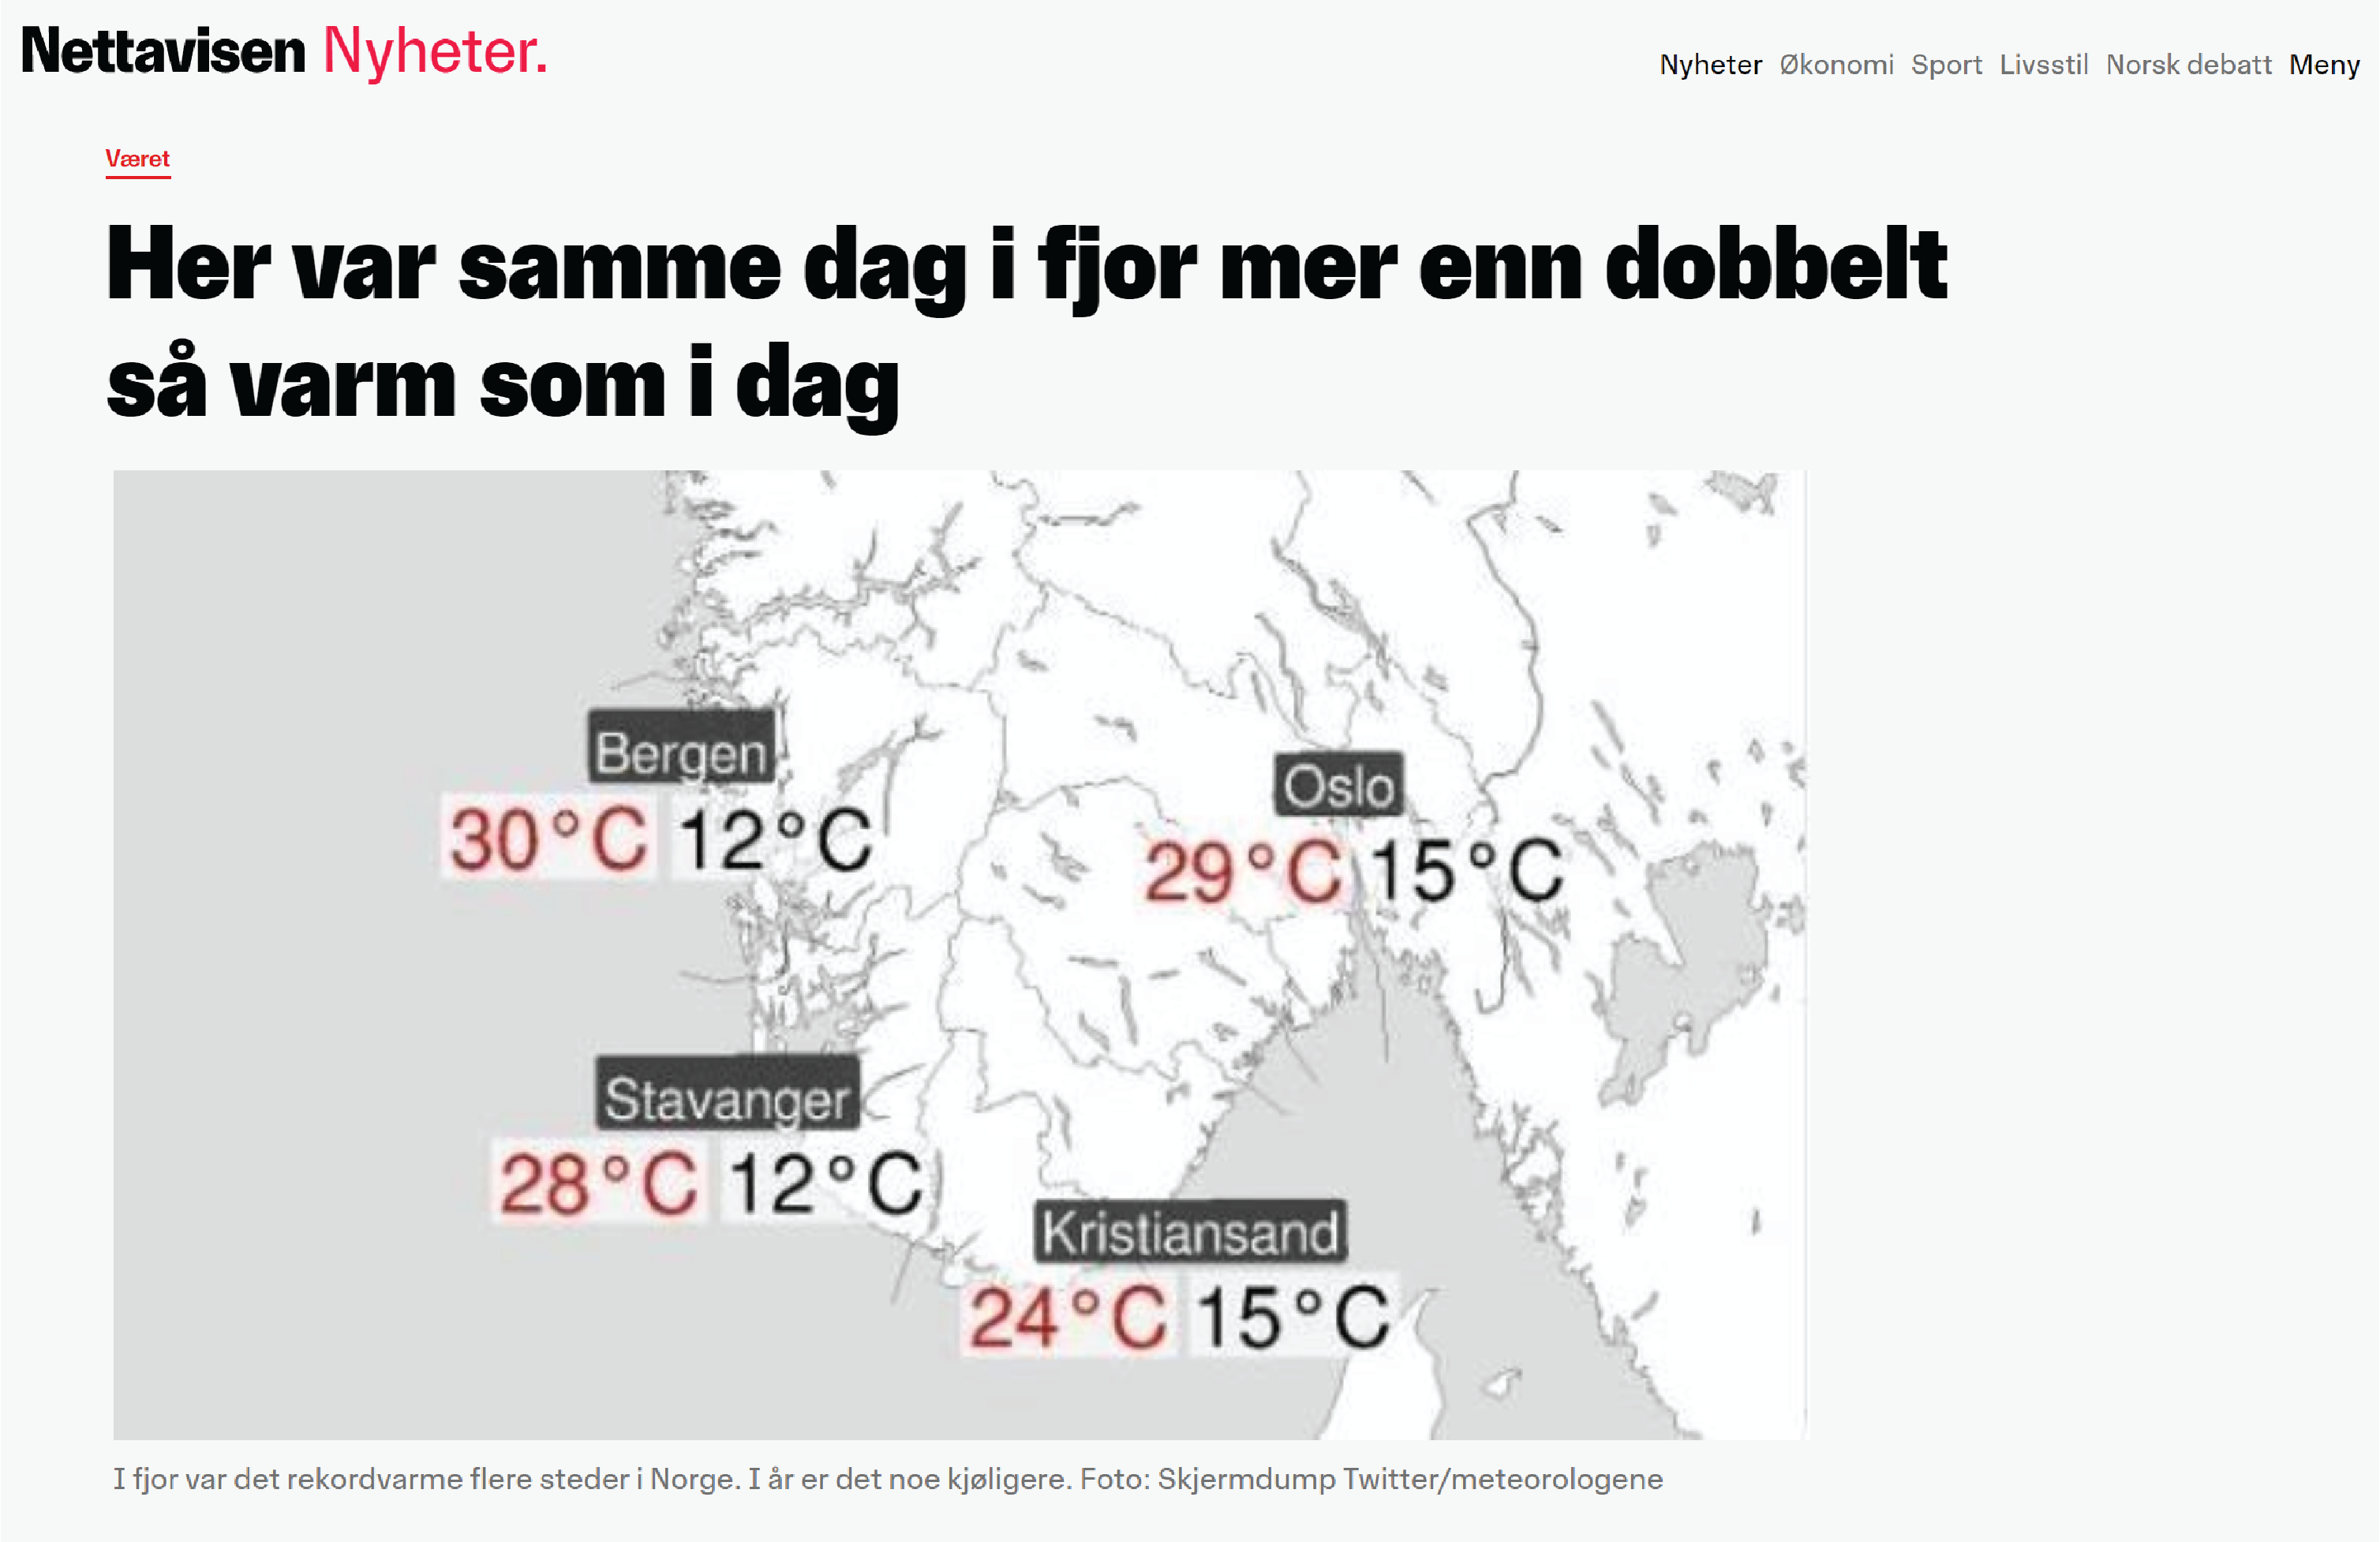
\includegraphics[width=9cm]{VarmeTemperaturFEIL}
\end{figure}




\newpage
\op[Med hjelpemidler]{6.1.1}{
Lufta består hovedsakelig av to-atomige gasser (hovedsakelig $N_2$).\\ \vsk

\oppg{a)}{Hva er gjennomsnittlige kinetiske energien til luft med temperatur 25$^\text{o}$C?}\vsk

I en liter med luft er det ca. 2,5 $\cdot$ 10$^{22}$ molekyler.\\ \vskk
\oppg{b)}{Hvor mye energi er det i én liter luft?}\vsk

I et klasserom er det ca. 140 000 liter med luft. Vi vil varme opp lufta i klasserommet fra  20$^\text{o}$C til 25$^\text{o}$C.\\ \vskk
\oppg{c)}{Hvor mye energi trenger vi?}\vsk

En varmeovn leverer 1000 J med varme hvert sekund til klasserommet.\\ \vsk
\oppg{d)}{Hvor lang tid bruker varmeovnen på å varme opp klasserommet?}
}




\op[Uten hjelpemidler]{}{
Den 18. mai 2024 hadde avisa \textit{Sør-Trøndelag} en artikkel med overskriften som er vist nedenfor.
\begin{figure}[H]
\centering

\includegraphics[width=8cm]{ST}
\end{figure}
Vanligvis er temperaturen omtrent 10$^\text{o}$C i Trøndelag på 17. mai.\\ \vskk

\oppg{a)}{Sett fra et fysikkperspektiv; Hvor høy temperatur er dobbelt så høy temperatur som 10$^\text{o}$C?}\vskk
\oppg{b)}{Kommenter avisa sin bruk av begrepet "varm".}

}
















\section{Trykk}

Trykk $P$ er kraft per areal,
\[  P = \frac{F}{A} \]
Trykk måles i Pa (pascal) og er det samme som N/m$^2$. \\ \vsk

Luftrykk kommer av at molekylene i lufta spretter rundt og dytter på omgivelsene. Hvor stort dette lufttrykket er, varierer med været (når det er fint vær er lufttrykket høyere enn når det er dårlig vær) og med høyden (det er lavere lufttrykk på en fjelltopp enn det er nede ved havet).\\ \vsk

Vanlig lufttrykk er ca. 101 kPa, altså ca. 101 kN per kvadratmeter.\\ \vsk

\eks[]{
En pult har et overflateareal på 1,0 m$^2$. Hvor stor masse tilsvarer kraften fra lufttrykket som presser pulten nedover?  \\ \vsk

\sv
Kraften blir
\[  F = P \cdot A = 101\; 325 \text{ N/m}^2 \cdot 1,0 \text{ m}^2 = 101 \; 325 \text{ N} \]
som tilsvarer en masse
\[ m = \frac{F}{g} = \frac{101 \; 325}{9,81} \approx \underline{\underline{10 \; 329 \text{ kg}}} \]
(Dette tilsvarer ca. 10 små biler)
\begin{figure}[H]
\centering
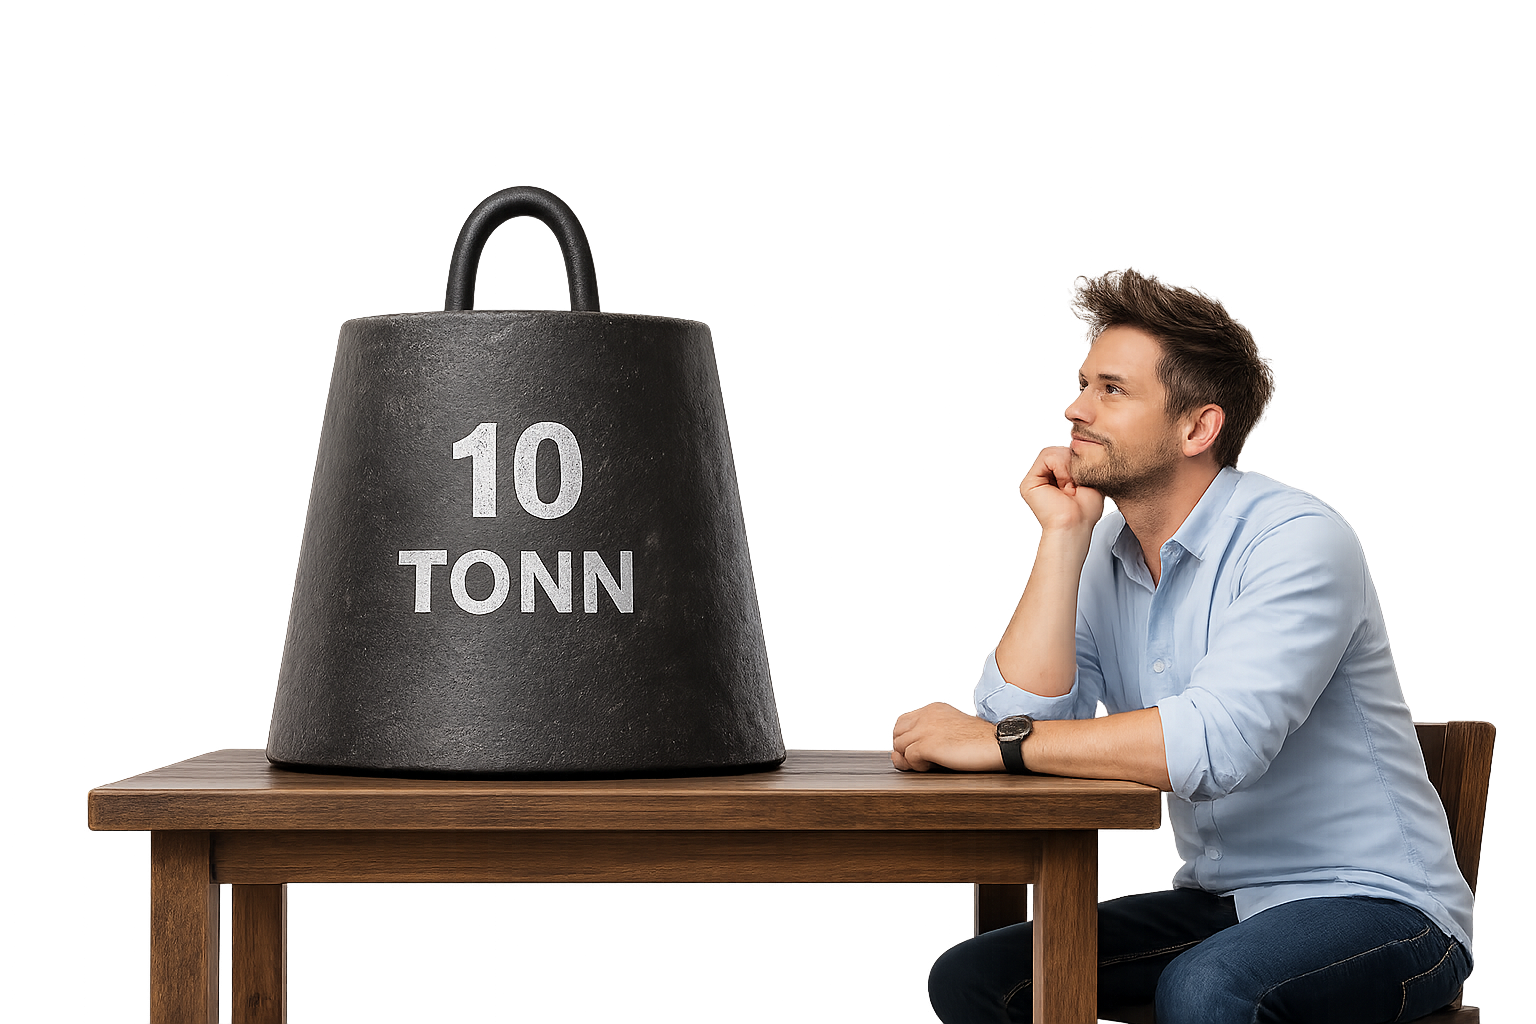
\includegraphics[width=5cm]{10Tonn}
\end{figure}
}



\newpage
\op[Med hjelpemidler]{6.2.1}{
Johanna har masse 35 kg og arealet av undersiden av føttene hennes er 0,022 m$^2$. Ina har masse 70 kg og arealet av undersiden av føttene hennes er 0,066 m$^2$.\\ \vskk

Hvem av dem opplever størst trykk mot undersiden av føttene når de står?
}


\op[Med hjelpemidler]{6.2.2}{
Lufttrykket er 101 kPa.

\oppg{a)}{Hvor stor kraft fra lufta virker på en vindusflate med overflateareal 0,50 m$^2$?}\vskk
\oppg{b)}{Hvorfor knuser ikke glasset?}
}


\op[Med hjelpemidler]{6.2.3}{
Formelen for vanntrykk $h$ meter under vannoverflaten er
\[ P_\text{vann} = \rho_\text{vann} \cdot g \cdot h \]
hvor tettheten til vann er $\rho_\text{vann}$ = 1000 kg/m$^3$.\\ \vskk
\oppg{a)}{Hvor mange meter under vann er vanntrykket 101 kPa?}\vsk

Når vi "suger" opp vann fra et sugerør skaper vi et lavere trykk inne i munnen enn på utsiden. Vannet suges egentlig ikke opp; Vannet dyttes opp av lufttrykket.
\begin{figure}[H]
\centering

\includegraphics[width=5cm]{brus}
\end{figure}
\oppg{b)}{Forklar at ikke det mulig å suge opp vann høyere enn 10,3 meter.}
}

















\section{Den ideelle gassloven}\label{PVnRT}

\textbf{Den ideelle gassloven} sier at
\[ PV = nRT \]
hvor $P$ er trykk, $V$ er volum, $n$ er antall mol i gassen, $T$ er temperatur og $R$ kalles gasskonstanten, og er gitt ved $R$ $=$ $8,314$ m$^2$ Pa / K mol. \\ \vsk

\eks[]{
En ballong har volum 1,0 liter når den er i romtemperatur. \\
Vi plasserer ballongen i et kjøleskap med temperatur 4,0 $^{\text{o}}$C. \\
Vi antar at lufttrykket er det samme i kjøleskapet som på utsiden. 
\begin{figure}[H]
\centering
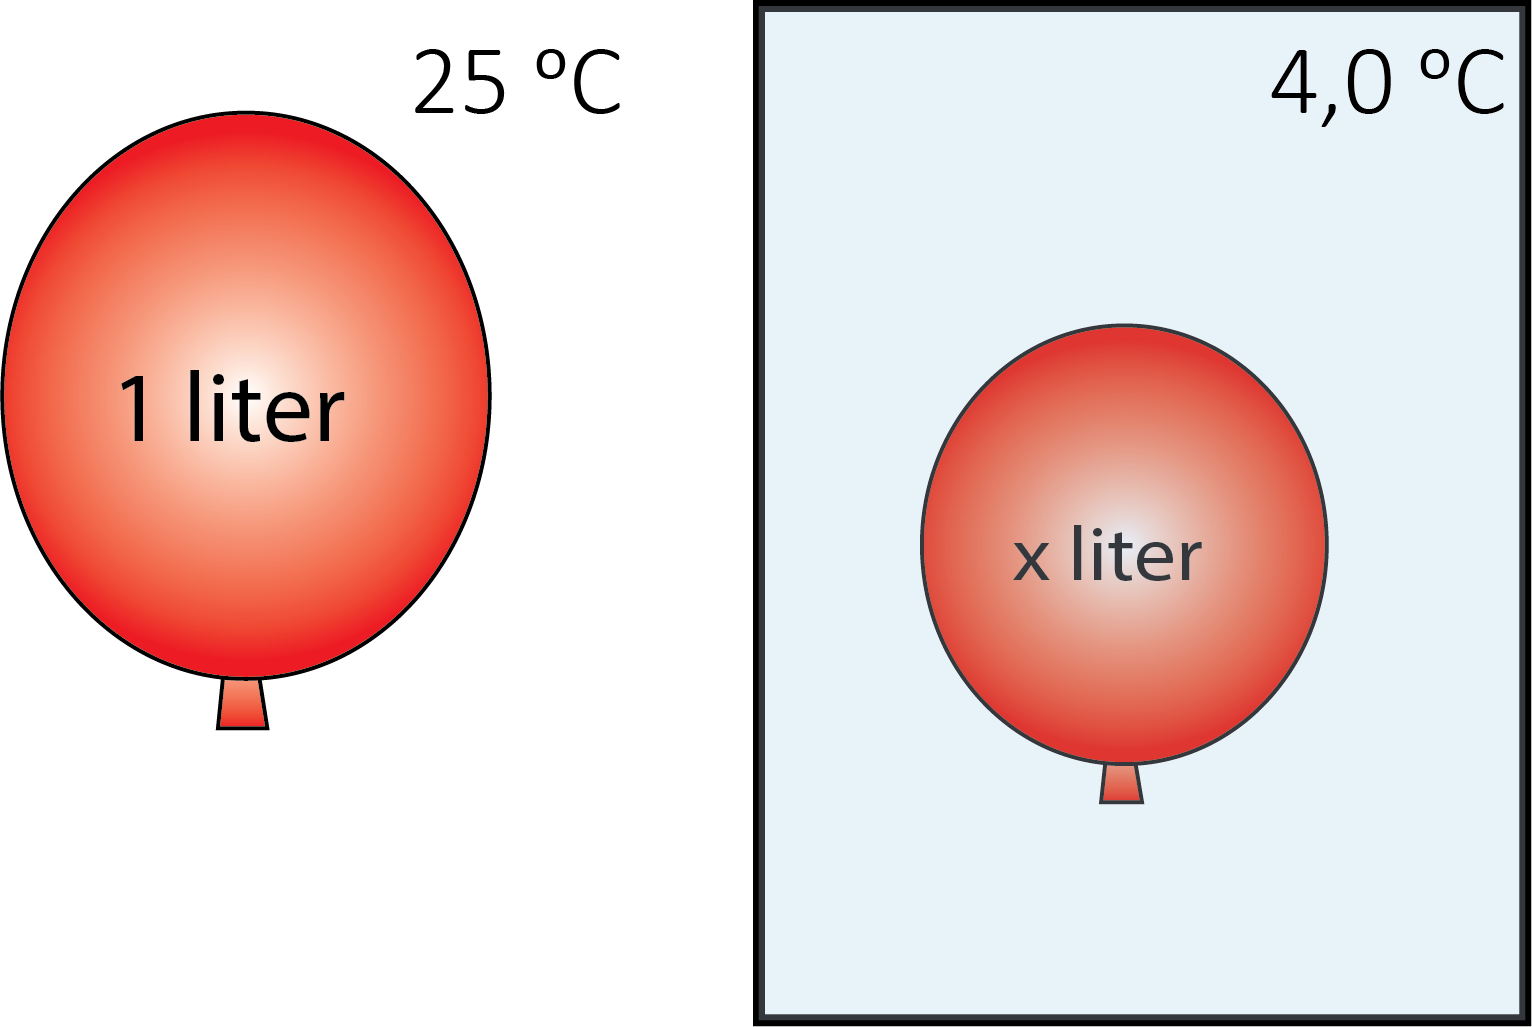
\includegraphics[width=5.5cm]{Ballong}
\end{figure}
Hvor stort volum får ballongen i kjøleskapet? \\ \vsk

\sv
\[ \frac{V_k}{V_0} = \frac{ \frac{nRT_k}{P} }{\frac{nRT_0}{P}} = \frac{T_k}{T_0} = \frac{277}{298} = 0,93 \;\; \Rightarrow \;\; x = \frac{277}{298} = \underline{\underline{0,93 \text{ liter}}} \]
}


\eks[]{
Vi bytter ut ballongen i eksempelet over med en termos.\\ \vsk

Hvor stort blir lufttrykket i termosen i kjøleskapet? \\ \vsk

\sv
\[ \frac{P_k}{P_0} = \frac{ \frac{nRT_k}{V} }{\frac{nRT_0}{V}} = \frac{T_k}{T_0} = \frac{277}{298} = 0,93 \;\; \Rightarrow \;\; P_k = 0,93 \cdot 101 \text{ kPa} = \underline{\underline{94 \text{ kPa}}} \]
}






\section{Termofysikkens 1. lov}

\textbf{Termofysikken 1. lov} sier at endringen av den indre energien $\Delta U$ til et system er
\[  \Delta U = Q + W \]
hvor $Q$  er varmeenergien \textit{tilført} systemet og $W$ er arbeidet som er gjort \textit{på} systemet. \\ \vsk


\textbf{Den indre energien $\Delta U$} består av
\begin{itemize}
	\item termisk energi (kinetisk energi til molekylene)
	\item kjemisk energi (energi i kjemiske bindinger)
\end{itemize}

Når ikke det skjer en faseovergang (is $\leftrightarrow$ vann $\leftrightarrow$ damp) er endringen av den indre energien endring av termisk energi. \\ \vsk

\eks[]{
En gass er stengt inne i en beholder med et lokk som kan flytte på seg. Et stearinlys tilfører en varme $Q$ = 2,00 kJ til gassen. Gassen bruker energien 0,50 kJ på å dytte lokket oppover. 
\begin{figure}[H]
\centering
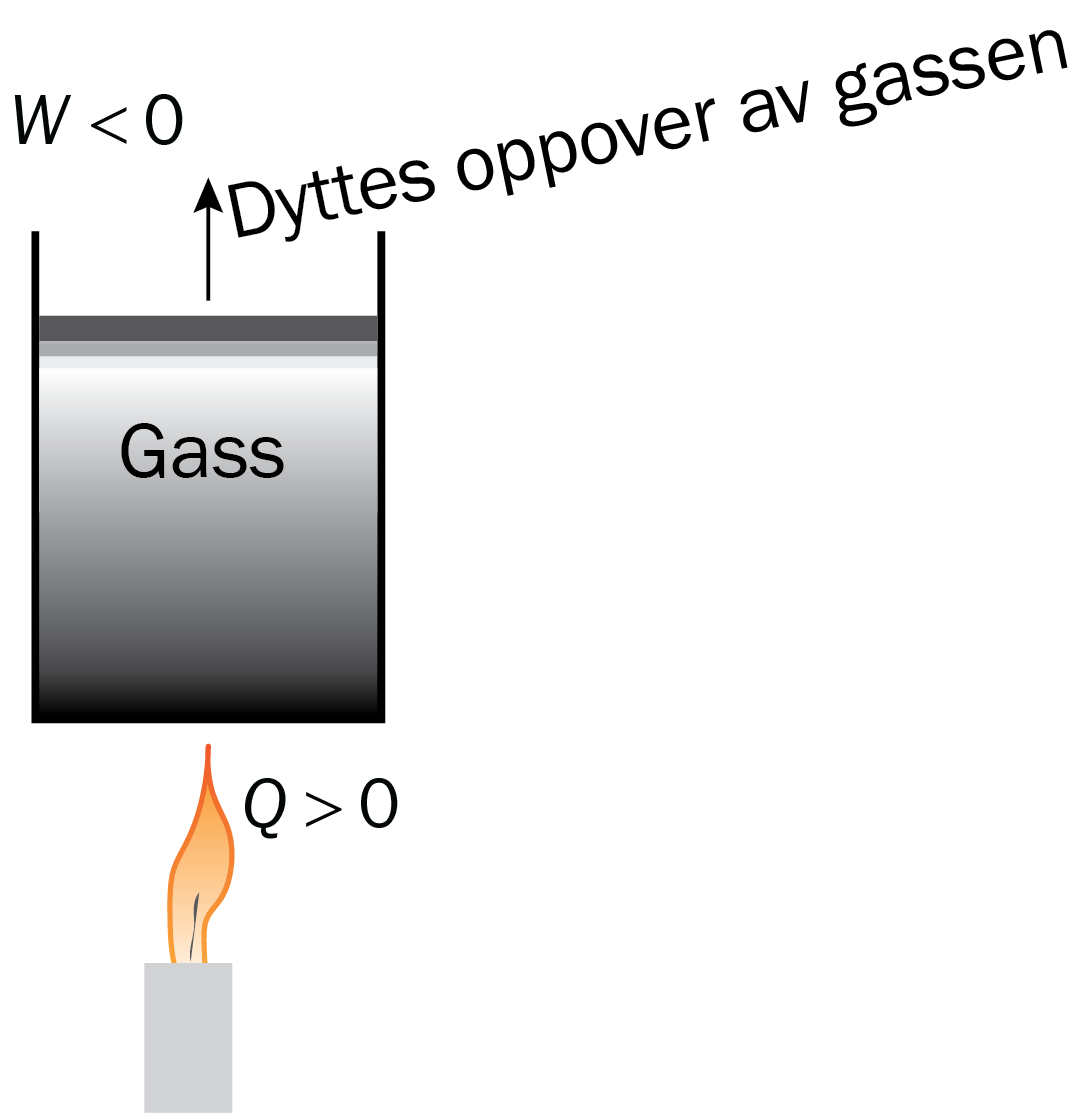
\includegraphics[width=4.5cm]{TD1L1}
\end{figure}

Hvor mye endres den termiske energien i gassen? \\ \vsk

\sv
\[ \Delta E_k = \Delta U = Q + W = 2,00 \text{ kJ} - 0,50 \text{ kJ} = \underline{\underline{1,50 \text{ kJ}}}   \]
}







\section{Termifysikkens 2. lov}

\textbf{Termofysikkens 2. lov} sier (noe så banalt som) at varme går fra et sted med høyere temperatur til et sted med lavere temperatur. \\ \vsk

\textbf{Termofysikkens 2. lov} kan også formuleres som at den totale \textbf{entropien} i alle prosesser øker. \\ \vsk

\begin{figure}[H]
\centering
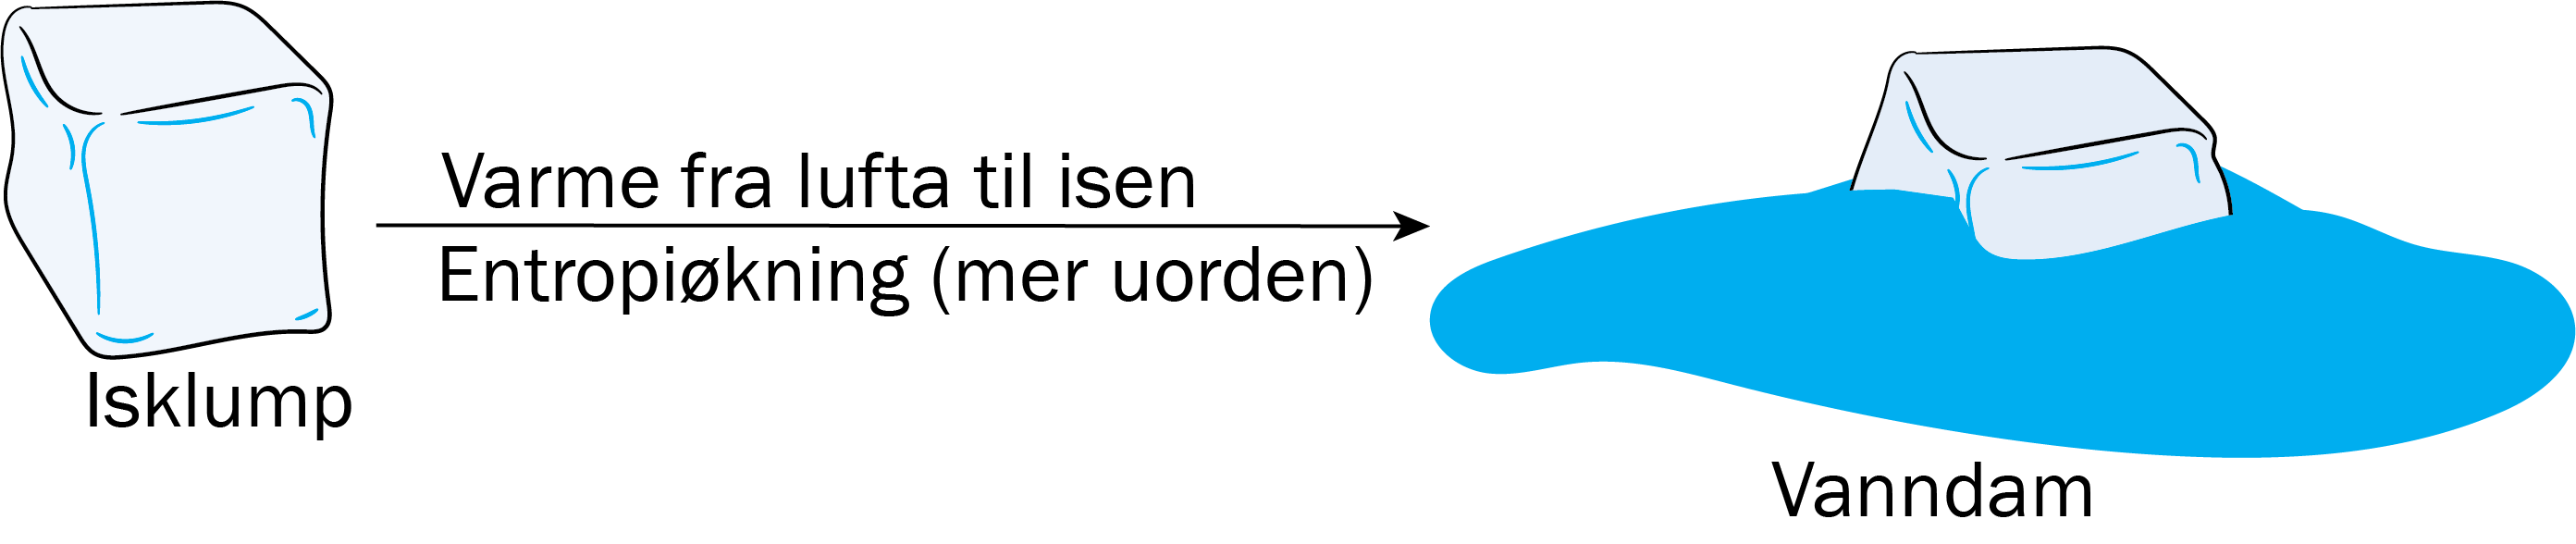
\includegraphics[width=11cm]{TD2L}
\end{figure}

\textbf{Entropi} er et mål på \textit{graden av uorden}. Fast stoff (is) har f.eks. mer orden enn flytende stoff (vann).\\ \vsk

Vi kan bruke termofysikkens 2. lov til å forklare hvorfor colaen blir kaldere når vi har isbiter i den; Varmen går bra colaen (varmere) til isbitene (kaldere). 
\begin{figure}[H]
\centering
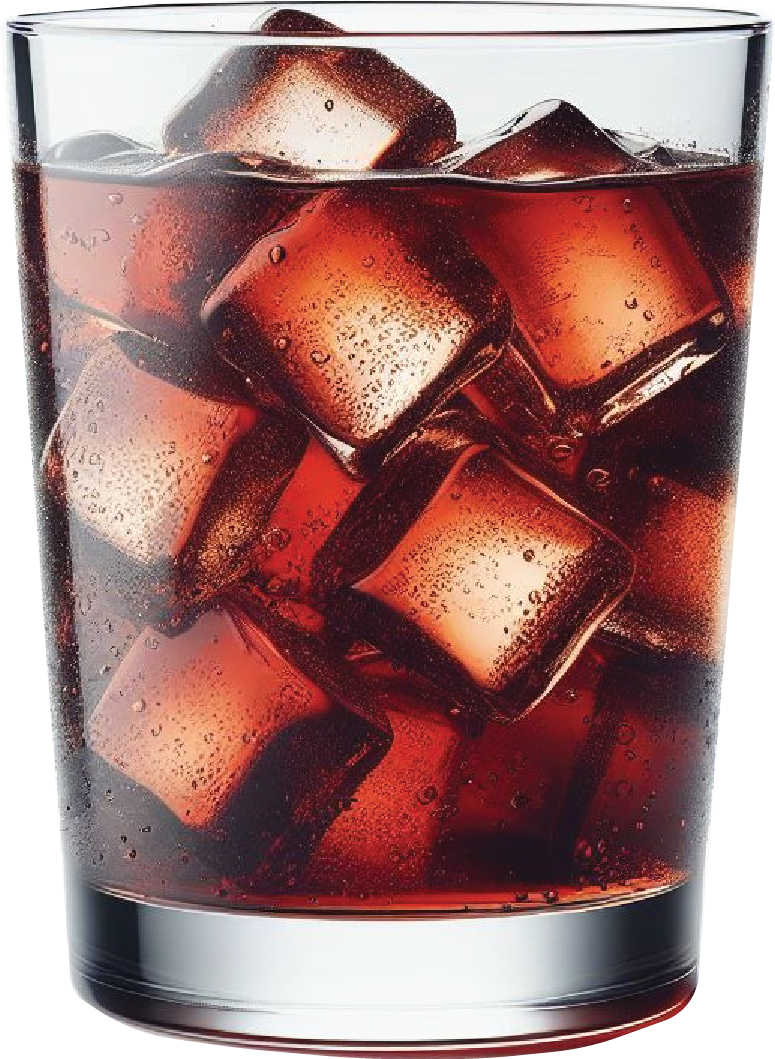
\includegraphics[width=2.5cm]{Cola100}
\end{figure}
I tillegg til å ta varme fra colaen for å bli varmet opp, tar også isbitene varme for å smelte. Faktisk tar faseovergangen \textit{is} $\rightarrow$ \textit{vann} mye mer varmeenergi fra colaen enn oppvarmingen av isbitene. For å forstå dette må vi se på varmekapasitet og faseoverganger (neste delkapittl).











\section{Varmekapasitet og faseoverganger}

\textbf{Spesifikk varmekapasitet} er energien vi må tilføre 1,0 kg av et stoff for å heve temperaturen 1 Kelvin (eller 1 $^{\text{o}}$C).\\ \vsk

\eks[]{
Vann har en spesifikk varmekapasitet på 4,1813 kJ/kg K.\\ \vsk

Hvor mye energi kreves for å varme opp 0,20 kg med vann fra 4,0 $^\text{o}$C til 90,0 $^\text{o}$C? \\ \vsk

\sv
\[ 4,1813 \text{ kJ/kg K} \cdot 0,20 \text{ kg} \cdot 86 \text{ K} = \underline{\underline{72 \text{ kJ}}} \]
}

\merk[]{Når vi regner med varmekapasitet er det lurt å ha med enhetene i utregningene. Ved å se på enehetene kan vi se om vi skal gange eller dele for å få det vi er ute etter.}

\textbf{Faseovergang} er at et stoff går fra en tilstand til en annen, f.eks. at vann går fra å være is til å bli flytende (eller omvendt), eller at vann går fra å være flytende til å blir vanndamp (eller omvendt). \\ \vsk

\textbf{Smeltevarme} er energien vi må tilføre 1,0 kg av et stoff for å smelte det, eller energien som frigjøres når 1,0 kg av et stoff fryser. \\ \vsk 

\textbf{Fordampingsvarme} er energien vi må tilføre 1,0 kg av et stoff for å fordampe det, eller energien som frigjøres når 1,0 kg av stoffet kondenserer. \\ \vsk 


\merk[]{Når vann tiner eller fordamper tar vannet varme fra omgivelsene.\\ \vsk

Når vann fryser eller kondenserer gir vannet varme til omgivelsene. }



\eks[]{
En isklump har masse 1,0 kg og temperatur -10 $^\text{o}$C. \\
Vi tilfører varme med en effekt på 1,0 kW = 1,0 kJ/s i 900 sekunder.\\ \vsk

Gitt følgende opplysninger:
\begin{itemize}
	\item Spesifikk varmekapasitet is: 2,05 kJ/kg K
	\item Spesifikk varmekapasitet vann: 4,18 kJ/kg K
	\item Smeltevarme is: 334 kJ/kg
\end{itemize}
\vsk

Beskriv sammenhengen mellom temperaturen og tid.\\ \vsk

\sv
Beregner tidsintervall for
\begin{itemize}
	\item oppvarming is: $2,05 \text{ kJ/kg K} \cdot 1,0 \text{ kg} \cdot 10 \text{ K} / 1,0 \text{ W} = 20,5 \text{ s}$
	\item smelting is: $334 \text{ kJ/kg} \cdot 1,0 \text{ kg} / 1,0 \text{ W} = 334 \text{ s}$
	\item oppvarming vann: $4,18 \text{ kJ/kg K} \cdot 1,0 \text{ kg} \cdot 100 \text{ K} / 1,0 \text{ W} = 418 \text{ s}$
\end{itemize}

\begin{figure}[H]
\centering
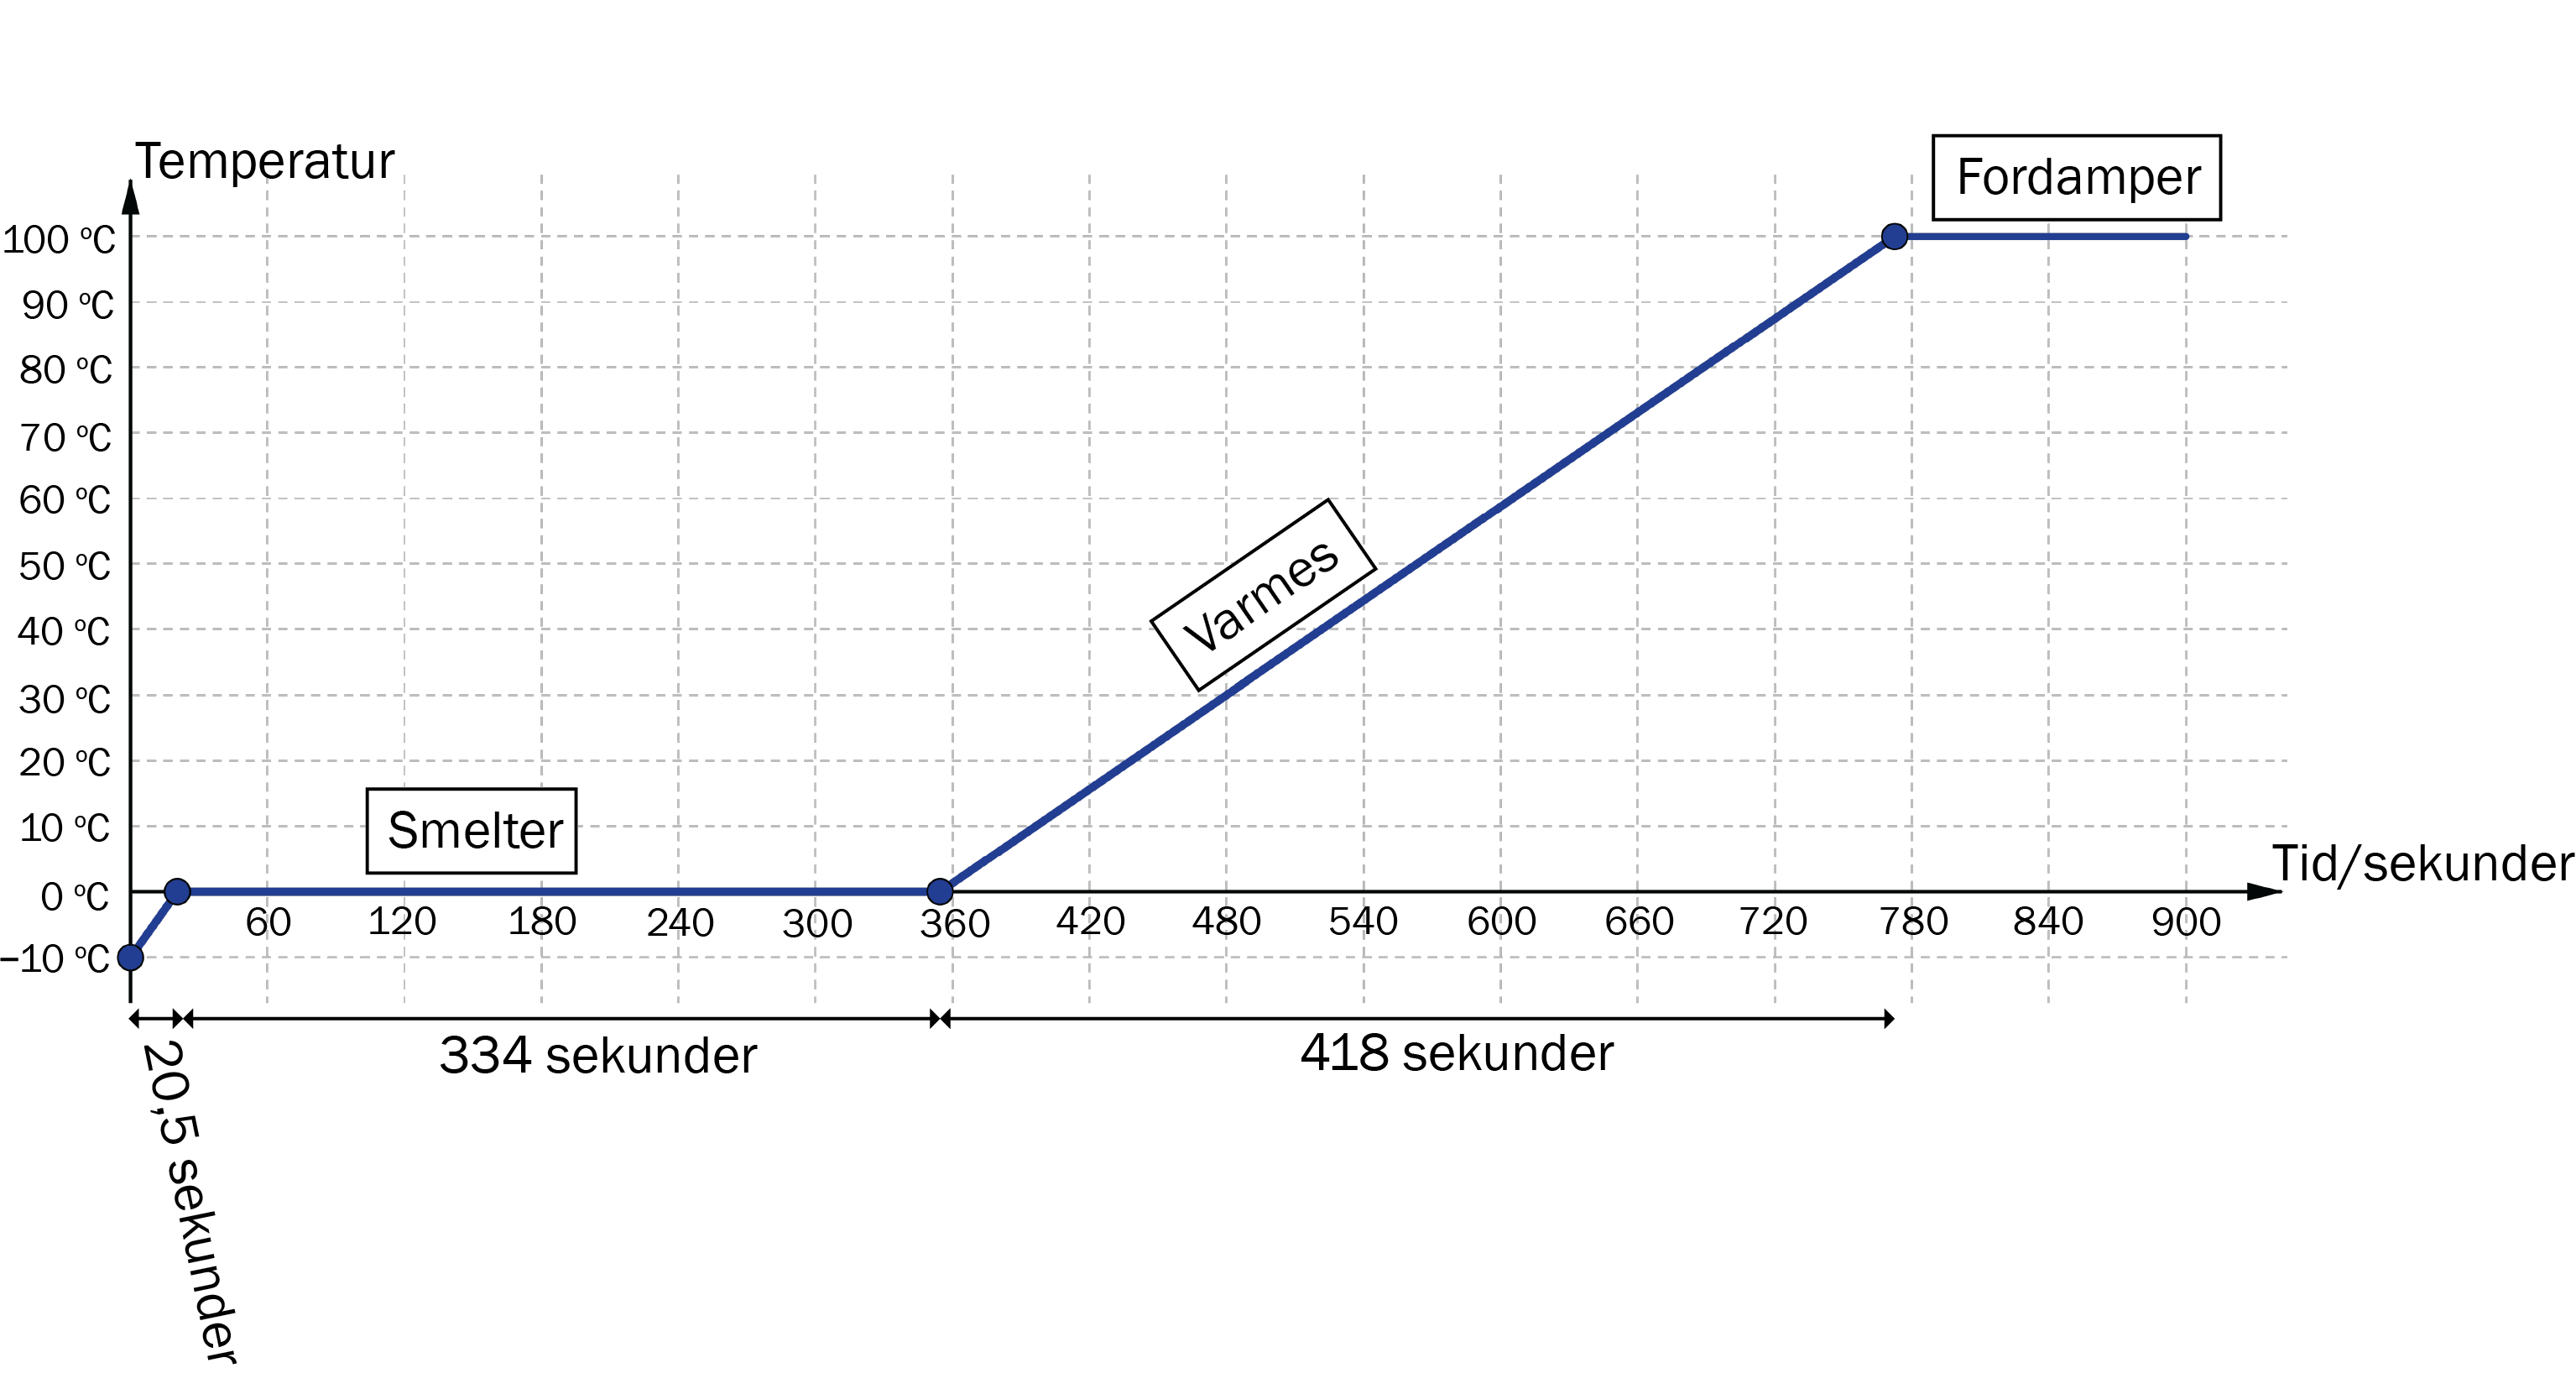
\includegraphics[width=11cm]{Faser2}
\end{figure}
}





\section{Virkningsgrad}

\textbf{Virkningsgrad} er definert som
\[\eta = \frac{P_{\text{nyttbar}}}{P_{\text{tilført}}} \]

\vsk

\eks[]{
Et lite badebasseng blir varmet opp av strålingen fra sola. Innstrålingen fra sola har en effekt på 700 W, virkningsgraden er 95 \% og det er 1000 kg med vann i bassenget.
\begin{figure}[H]
\centering

\includegraphics[width=4cm]{Basseng}
\end{figure}

Hvor mye stiger temperaturen til vannet i løpet av 10 timer?\\ \vsk

\sv
Energien som varmer opp vannet blir
\[ E = \eta \cdot P \cdot t = 0,95 \cdot 700 \text{ J/s} \cdot 10 \cdot 60 \cdot 60 \text{ s} = 23940 \text{ kJ} \]
Den spesifikke varmekapasiteten for vann 4,18 kJ/kg $^\text{o}$C gir
\[ \Delta T = \frac{23940 \text{ kJ}}{4,18 \text{ kJ/kg $^\text{o}$C} \cdot 1000 \text{ kg}} = 5,8 \text{ $^\text{o}$C} \]
}












\end{document}